\documentclass[../main.tex]{subfiles}

\begin{document}

\chapter{Results}
The software module developed in this project does not fulfill all requirements (see appendix \ref{appendix-specification}), in that it does not handle \textit{conditional restrictions} at all, and not all implemented restrictions are handled correctly, see section \ref{sect:result-specification} below.

But the software does build a \textit{line graph} that can be fetched and stored in database for inspection with visual tools, see section \ref{sect:result-visual} below.

The project has so far been about implementing things and have not had any focus on performance, but some performance tests have been run, see section \ref{sect:result-performance}.

% ======================================================================================
\section{Specification fulfillment}\label{sect:result-specification}
Table \ref{table:specification-fulfillment} shows how much of the specification that has been fulfilled.

\begin{table}[h]
\centering
\caption{Fulfillment of specification.}
    \begin{tabular}{|r|c||l|}
    \hline
    Section & Fulfills & Comment \\
    \hline
    \hline
    \multicolumn{3}{|l|}{1.2 Main use case} \\
    \hline
    1.2.1 & X & As call to \texttt{LineGraphUtility::getLineGraph()}. \\
    \hline
    1.2.2 & X & \\
    \hline
    1.2.3 & X & \\
    \hline
    1.2.4 & X & \\
    \hline
    \multicolumn{3}{|l|}{1.3 Optional use case} \\
    \hline
    1.3.1 & X & \\
    \hline
    1.3.2 & X & \\
    \hline
    \multicolumn{3}{|l|}{1.4 Functional requirements} \\
    \hline
    1.4.1 & & Lots of work remains to implement all restrictions. \\
    \hline
    1.4.2 & X & \\
    \hline
    1.4.3 & X & \\
    \hline
    1.4.4 & X & Some small parts are hard coded. \\
    \hline
    \multicolumn{3}{|l|}{1.5 Non-functional requirements} \\
    \hline
    1.5.1 & X & Written in C++. \\
    \hline
    1.5.2 & X & Did not find pgRouting really useable. \\
    \hline
    \multicolumn{3}{|l|}{1.6 Testing requirements} \\
    \hline
    1.6 & X &  \\
    \hline
    \multicolumn{3}{|l|}{1.7 Coding standard} \\
    \hline
    1.7 & X & \\
    \hline
    \end{tabular}
\label{table:specification-fulfillment}
\end{table}

% ======================================================================================
\section{Visual examination}\label{sect:result-visual}

Maps are easy to visualize, and a great number of tools exist to work with map data. Figure \ref{fig:mikh-osm-maps} shows a piece of a map over Mikhailovsk. In order to test if the handling of restrictions work, modified maps have been created. \textit{JOSM}\footnote{\url{https://josm.openstreetmap.de/}} is a tool for manipulating \textit{OSM} data. In figure \ref{fig:mikh-osm-map-barrier} it is indicated where a \textit{bollard barrier} has been added in the middle of a road, just to see if the restrictions work, and the new map is saved in its own \texttt{.osm} file, and a new database built for it. 

\begin{figure}[h]
    \centering
    \begin{subfigure}[t]{0.4\linewidth}
        \centering
        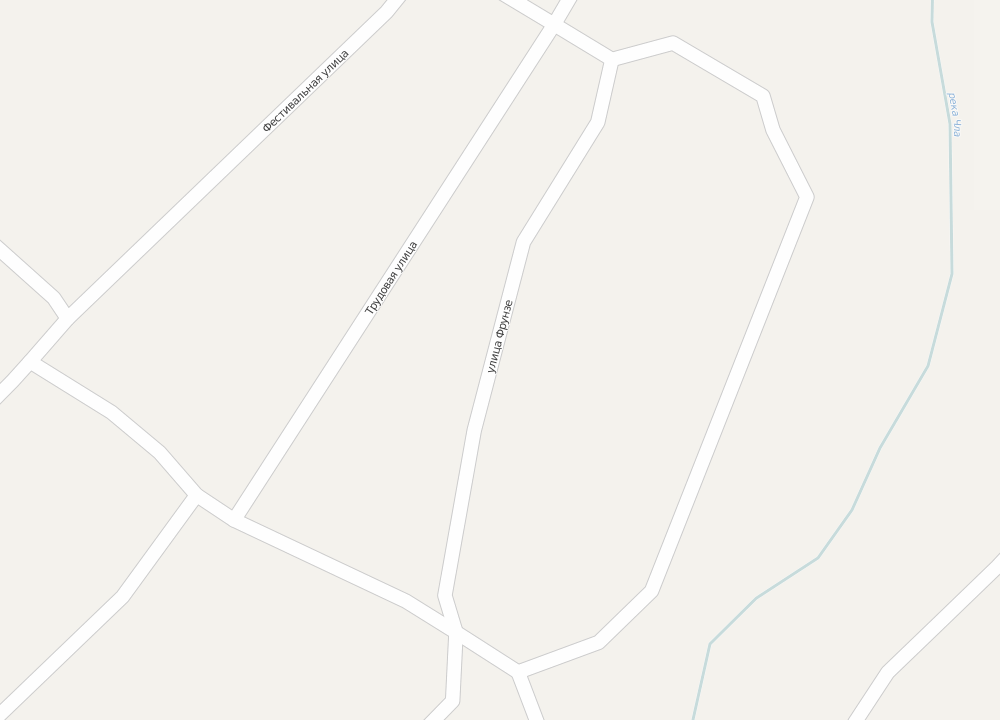
\includegraphics[width=\linewidth]{mikh-osm-map}
        \caption{Original.}
        \label{fig:mikh-osm-map-orig}
    \end{subfigure}
    \hspace{5mm}
    \begin{subfigure}[t]{0.4\linewidth}
        \centering
        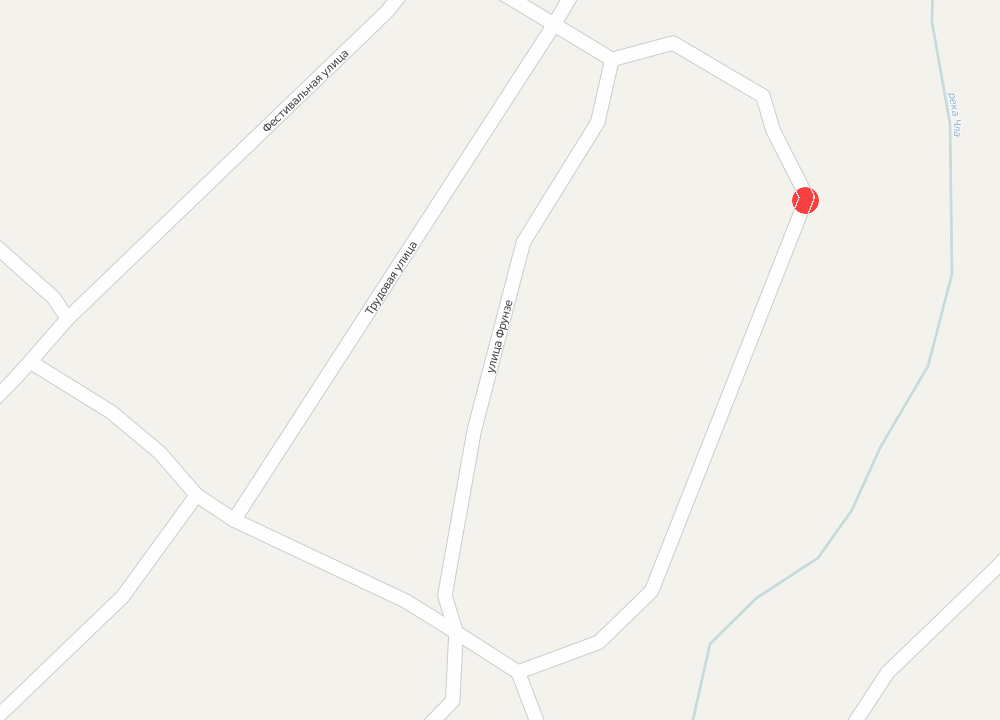
\includegraphics[width=\linewidth]{mikh-osm-map-barrier}
        \caption{Modified with added barrier.}
        \label{fig:mikh-osm-map-barrier}
    \end{subfigure}
    \caption{Map over part of Mikhailovsk. \cite{img-mikh-osm-map}}
    \label{fig:mikh-osm-maps}
\end{figure}

Using another tool, \textit{QGIS}\footnote{\url{http://www.qgis.org}} can be used to load map data from for example a \textit{PostGIS} database and viewed. In figure \ref{fig:mikh-osm-map-topo} the vertices and edges from the topology for that map has been layered on top of the image (with a slight misalignment). The topology is the same for both maps, it does not change with added barriers.

\begin{figure}[h]
    \centering
    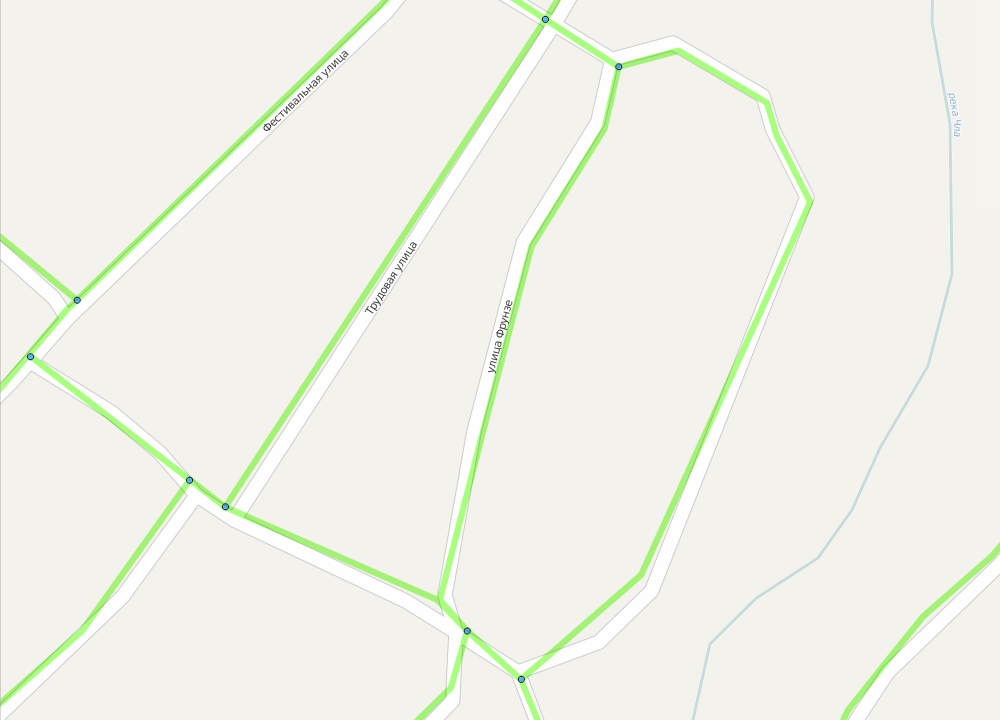
\includegraphics[width=0.8\linewidth]{mikh-osm-map-topo}
    \caption{Edges (green) and vertices (blue) for the topology.}
    \label{fig:mikh-osm-map-topo}
\end{figure}

The interesting part is to see if the restriction has had any impact on the built \textit{line graph}, see figure \ref{fig:mikh-osm-map-orig-linegraph} for the original line graph, where the road is included in the line graph. It has a \textit{node} in the middle and \textit{lines} connecting to the adjacent \textit{edges/nodes}.

Figure \ref{fig:mikh-osm-map-barrier-linegraph} shows the line graph after the restricting barrier has been added to the map. There one can see that the \textit{edge} (road) has not been added as a \textit{node} to the line graph, while all the other \textit{lines} and \textit{nodes} remain the same. This practically disables routing along that road.

\begin{figure}[H]
    \centering
    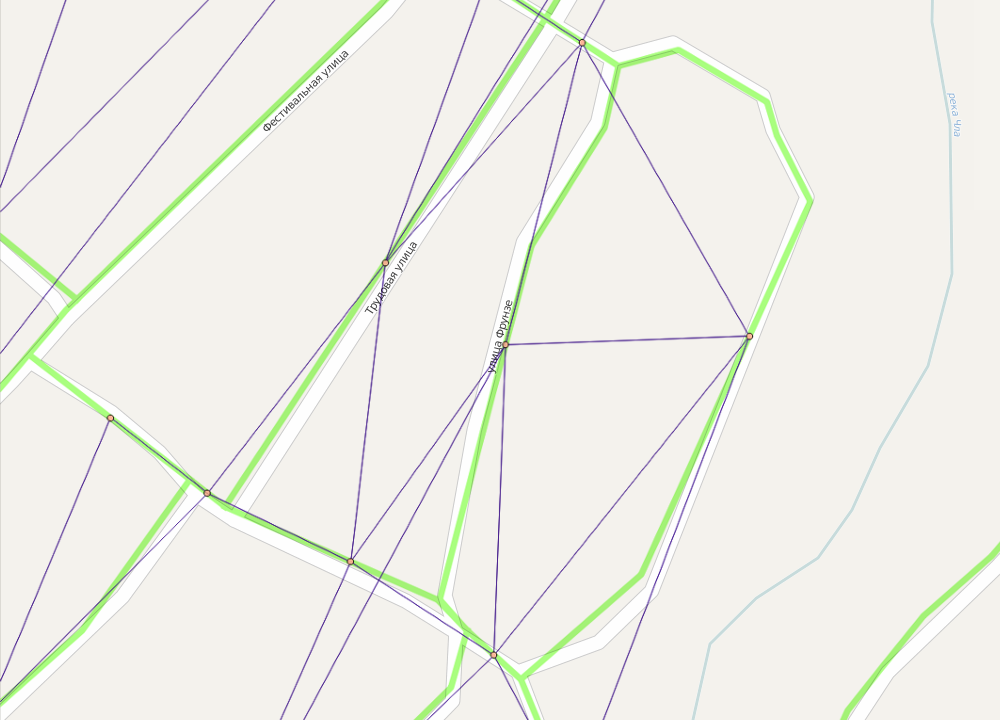
\includegraphics[width=0.8\linewidth]{mikh-osm-map-orig-linegraph}
    \caption{Original \textit{line graph}. \textit{Lines} in purple.}
    \label{fig:mikh-osm-map-orig-linegraph}
\end{figure}

\begin{figure}[H]
    \centering
    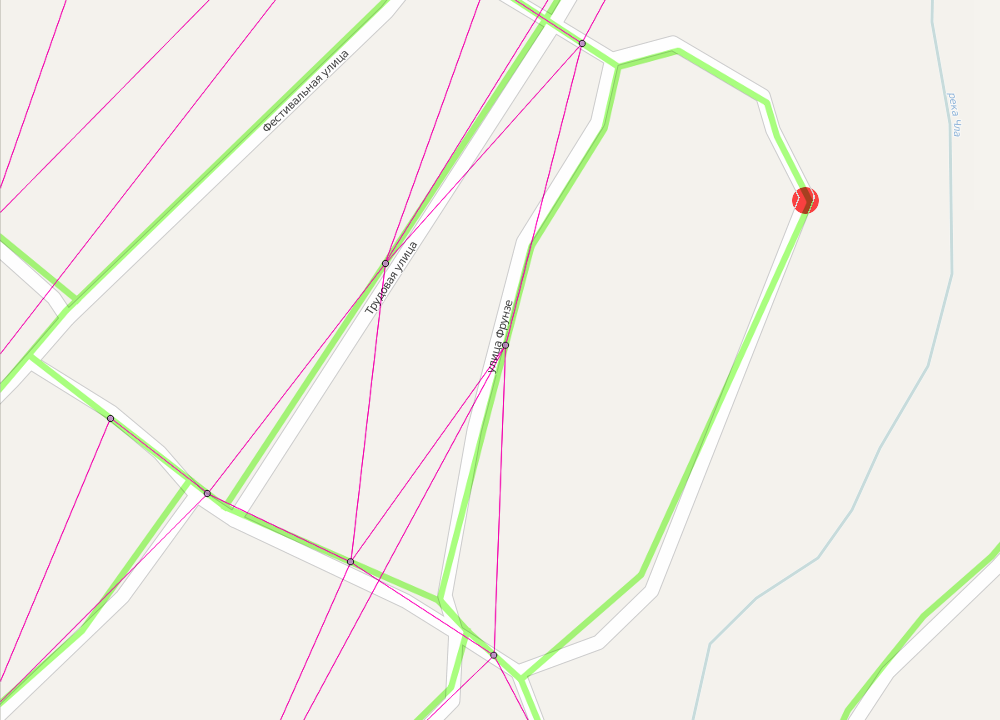
\includegraphics[width=0.8\linewidth]{mikh-osm-map-barrier-linegraph}
    \caption{\textit{Line graph} after added barrier. \textit{Lines} in magenta.}
    \label{fig:mikh-osm-map-barrier-linegraph}
\end{figure}


% ======================================================================================
\section{Performance}\label{sect:result-performance}
There were \textit{soft real time} requirements in the specification, but they were not specified more than that. But it is interesting so find out how long it takes to fetch a \textit{line graph}, built on demand by the software module.

A few test cases were written in \texttt{LineGraphUtility\_test.cc} that averages the number of \textit{microseconds} it takes to instantiate a \texttt{LineGraphUtility} and fetch a \textit{line graph}, over a given number of rounds.

The test runs on both a configuration with a pre-built topology, and a configuration that builds a temporary topology.

See table \ref{table:test-results} for test results.

\begin{table}[h]
\centering
\caption{Time in $\mu$s to fetch a \textit{line graph}, with pre-built versus temporary topologies.}
    \begin{tabular}{|c|l|r|r|r|r||r|}
    \hline
    \multicolumn{2}{|r|}{Test \#} & 1 & 2 & 3 & 4 & Sum \\
    \hline
    \hline
    \multicolumn{2}{|r|}{\# of rounds} & 10 & 10 & 10 & 70 & 100\\
    \hline
    \multicolumn{2}{|c||}{topology} & avg ($\mu$s) & avg ($\mu$s) & avg ($\mu$s) & avg ($\mu$s) & avg ($\mu$s) \\
    \hline
    \hline
    \multirow{2}{5em}{Mikhailovsk} & normal & 147859 & 149092 & 141782 & 133950 & 143171 \\
     & temporary & 5026626 & 4924245 & 4917319 & 4875838 & 4936007 \\
    \hline
    \multirow{2}{5em}{Partille} & normal & 180340 & 188405 & 179883 & 179978 & 182152\\
     & temporary & 10683194 & 10342420 & 10683873 & 10521535 & 10557756\\
    \hline
    \end{tabular}
\label{table:test-results}
\end{table}

The \textit{size} (number of edges) and \textit{order} (number of vertices) of the graphs are shown in table \ref{table:graph-sizes}.

\begin{table}[h]
\centering
\caption{Sizes of tested graphs}
    \begin{tabular}{|c|r|r|r|r|}
    \hline
     & \multicolumn{2}{c|}{Graph} & \multicolumn{2}{|c|}{Line graph}  \\
    \hline
     & vertices & edges & nodes & lines \\
    \hline
    \hline
    Mikhailovsk & 654 & 1618 & 1618 & 4758 \\
    \hline
    Partille & 1645 & 2265 & 2265 & 5577 \\
    \hline
    \end{tabular}
\label{table:graph-sizes}
\end{table}

The results shows that, in order to meet \textit{soft real time requirements} it is not possible to build temporary topologies at every instantiation of a \texttt{LineGraphUtility}, as the time increases dramatically. In the case of \textit{Mikhailovsk}, the increase is from 0.14 s to 4.93 s, about 34 times as much. In the case of \textit{Partille}, the increase is from 0.18 s to 10.55 s, nearly 58 times. 

That fetching a line graph with a pre-built topology takes 0.15-0.2 s might fall within the requirements.

The test were conducted on a computer with 8 GB ram, processor Intel i7-4702MQ, running Linux Mint 17.1 with Linux kernel version 3.13.0-37-generic. The comiler flags were the same as for the rest of the project, i.e. no optimization.


\end{document}